\documentclass[12pt,letterpaper]{article}

\usepackage{quiver}
\usepackage{Pack}
\usepackage{PackMath}
\usepackage[placement=bottom,angle=0,color=black!40,scale=3,hshift=88,vshift=5]{background}
\usepackage{enumitem}
\setlist{nosep}
\usepackage{hyperref}
\usepackage{cleveref}
\usepackage{makecell}
\graphicspath{{./imgs/}}

\usepackage{minted}
\newcommand{\code}[1]{\texttt{#1}}
% \newenvironment{codeblock}{\VerbatimEnvironment \begin{minted}[linenos,breaklines]{python}}{\end{minted}}


\backgroundsetup{contents={-\thepage-}}
\makeatletter
\renewcommand*\env@matrix[1][*\c@MaxMatrixCols c]{%
   \hskip -\arraycolsep
   \let\@ifnextchar\new@ifnextchar
   \array{#1}}
\makeatother

\usepackage{fancyhdr}
\pagestyle{fancy}
\fancyhf{}
\fancyhead[LE,RO]{Workshop 2}
\fancyhead[CE,CO]{Yuxi (Jaden) Long}
\fancyhead[RE,LO]{Duke BioByte}
%\fancyfoot[CE,CO]{}

% For progress tracker
\newcommand{\ns}{{\color{red} Not Started}}
\newcommand{\ip}{{\color{orange} In Progress (Stuck)}}
\newcommand{\td}{{\color{blue} In Progress (To-Do)}}
\newcommand{\fin}{{\color{green} Finished}}
\newcommand{\qm}{{\color{violet} Finshed, But In Doubt}}
\newcommand{\contradiction}{\Rightarrow\!\Leftarrow}
\renewcommand{\im}{\mathrm{im\,}}
\renewcommand{\tilde}{\widetilde}
\setlength{\parindent}{0em}
\setlength{\parskip}{0.5em}


\usepackage{notomath}
\usepackage{multicol}
\newcommand{\Hint}{\textcolor{violet}{\textit{Hint: }}}
\newcommand{\Solution}{\textcolor{MidnightBlue}{\textbf{Solution: }}}


\title{\textbf{Sequence Alignment and Variant Calling}}
\author{\textit{Computational Tools for the Working Biologist. Workshop 2}}
\date{Yuxi (Jaden) Long}

\begin{document}
\maketitle
\thispagestyle{empty}

\vspace{1em}

\noindent
Short-read DNA or RNA sequencing is cheap and fast, and generates a lot of data. As a result, genomics is the most relevant and fundamental computational task that a biologist would encounter.

\noindent
\textbf{Central idea/technique:} Understand the information in genomic sequencing raw data, and learn tools to manipulate them.

\textbf{Practice:} Perform variant calling on a sequencing datum from beginning to end.

\begin{itemize}
   \item Quality control: fastp
   \item Reference data: NCBI GenBank, NCBI SRA
   \item Reference based sequence alignment: BWA
   \item Viewing your alignment: IGV
   \item Alignment processing: samtools, picard
   \item Variant calling: GATK HaplotypeCaller
\end{itemize}

\textit{This workflow is largely adapted from the independent study of Hector de Galard in Fall 2019 (\href{https://github.com/longyuxi/biobyte-bioinformatics-workshop/blob/main/2/supplement/Hector_19L22.docx}{his report}), and the \href{https://www.hadriengourle.com/wrangling-genomics/01-variant_calling_workflow/}{Wrangling Genomics workshop} by Data Carpentry.}

\section{Short read sequencing}

You have probably heard of Sanger sequencing from biology class. Sanger sequencing is considered the ``first generation'' of sequencing technologies. Later technologies improved on the \textit{throughput}, which is the amount of data generated per sequencing run, and the large amount of data generated allowed for amazing new research insights made by researchers around the world, but also necessitated the use of bulk data processing tools.

In principle, genome sequencing can be considered as measuring the nucleotide sequences of fragments that come the genome of interest. Each such measurement is called a \textit{read}. Naturally, each read is associated with a \textit{read length}, which is the length of each fragment sequenced, measured in base pairs. Characterized by their read lengths, the generation of sequencing technologies that boomed in the 2000s and early 2010s are called ``short-read sequencing'', and in the past decade we saw the development of ``long-read sequencing''. Below, you can find a table to overview these technologies. Note that I am not distinguishing between DNA and RNA sequencing -- the same technologies are used for both types of nucleic acids, as transcription and reverse transcription allows one to convert from one type to the other.

Another important metric for genome sequencing is \textit{read depth}. The read depth of a certain base in the genome is the number of reads covering that base. As you may have guessed by now, we have the following formula:

\begin{table}
\begin{center}
\begin{tabular}{|l|l|l|}
\hline
\makecell{\textbf{Sequencing technologies}} & \makecell{\textbf{Short-read}} & \makecell{\textbf{Long-read}} \\ \hline
\makecell{\textbf{Currently prominent companies}} & \makecell{Illumina, Element Bio} &  \makecell{Oxford Nanopore, PacBio}  \\ \hline
\makecell{\textbf{Read length}} & \makecell{Up to 2 $\times$ 300 bp} &  \makecell{N50 $\sim$25 kb (Nanopore) \\ 10--25 kb (PacBio)}  \\ \hline
\makecell{\textbf{Other name}} & \makecell{Next generation sequencing} & \makecell{Third generation sequencing}   \\ \hline
\makecell{\textbf{Cost per base}} & \makecell{Relatively cheaper} & \makecell{Relatively more expensive}   \\ \hline
\end{tabular}
\end{center}
\caption{The most important differences between short-read and long-read sequencing technologies. \textbf{Disclaimer:} This list is meant to give an idea of the current technologies on the market and is by no means comprehensive. Read lengths differ between different platforms within the same company. Do your own research.}
\end{table}

\begin{figure}
\centering
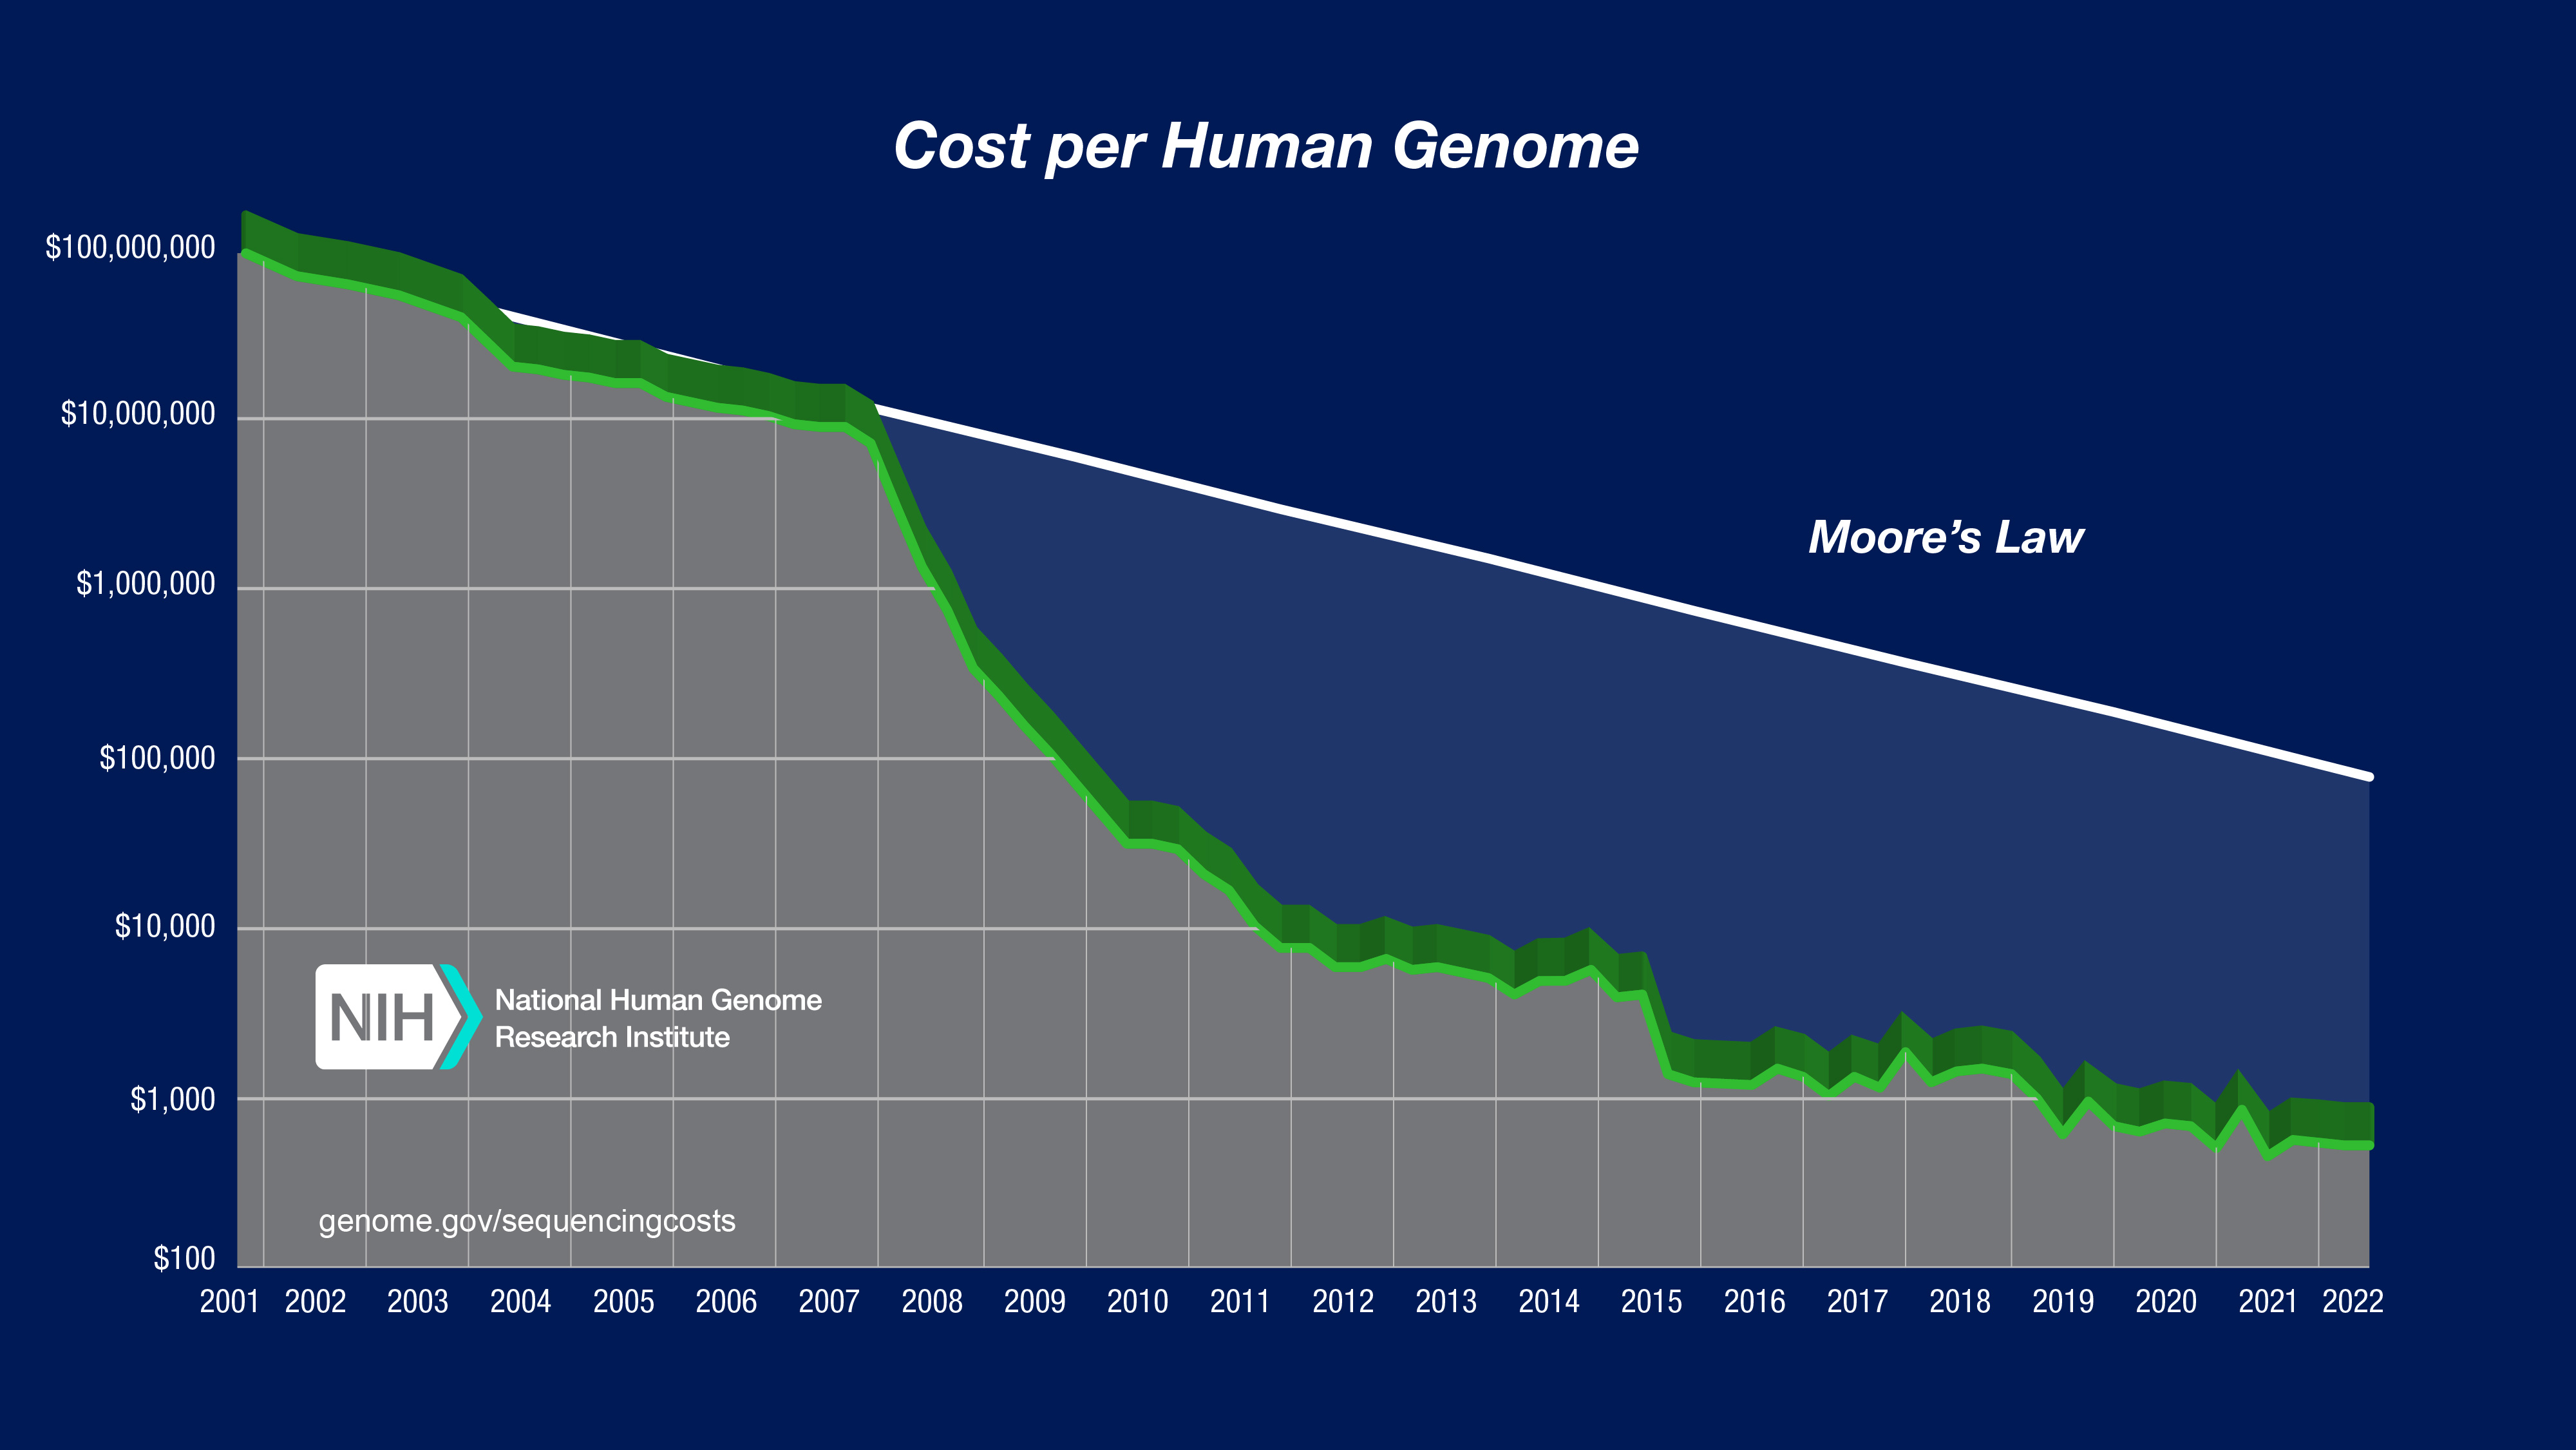
\includegraphics[width=0.8\textwidth]{genome_sequencing_cost.jpg}
\caption{Sequencing cost has dropped rapidly in the past two decades. Source: \href{https://www.genome.gov/about-genomics/fact-sheets/Sequencing-Human-Genome-cost}{NIH}. This is largely due to advances in next generation sequencing.}
\label{fig:genome-sequencing-cost}
\end{figure}

Short-read sequencing is cheap. But there is a catch. Its short read length fundamentally limits the types of analyses that can be done on it. Just from the sequencing results, one cannot distinguish repeats of a genomic region that are longer than the read length. That means no tandem repeats. The first telomere-to-telomere sequence of the human genome was only published in 2022 (\href{https://www.science.org/doi/10.1126/science.abj6987}{Nurk et al., 2022}). On the other hand, short read sequencing is effective determining RNA expression, especially fueled by recent advances in spatial transcriptomics and single cell transcriptomics, which are essentially pre- and post-processing technologies layered on top of the existing sequencing platforms. In this workshop, we shall focus on variant calling, which is the process of identifying genomic mutations, from short-read sequencing data.

\section{The variant calling workflow}

The heart of variant calling is to compare our sequencing data to a \textit{reference genome}. We wish to first \textit{align} each of our sequencing reads to the reference genome (that is, find our where that read most likely belongs, given there could be a few mutations). There are some processing steps for quality control before and after alignment. Then, \textit{variant calling} is done on the aligned reads, which finds the mutations we are after.

A simplified workflow, which we will follow, can be found in \cref*{fig:simplified-varcall-workflow}. The full best practices workflow from the developers of Genome Analysis Toolkit (GATK) can be found in \cref*{fig:gatk-varcall-workflow}. The hope is that, in practicing and understanding this basic workflow, you will be able to perform a basic analysis from beginning to end. When you are dexterous with this workflow, you can also add more moving parts to it without being overwhelmed.

\begin{figure}[H]
\centering
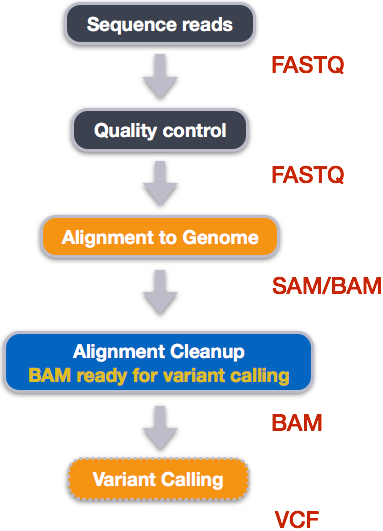
\includegraphics[width=0.3\textwidth]{data_carpentry_variant_calling_workflow.png}
\caption{Simplified variant calling workflow, from Data Carpentry.}
\label{fig:simplified-varcall-workflow}
\end{figure}

\begin{figure}[H]
\centering
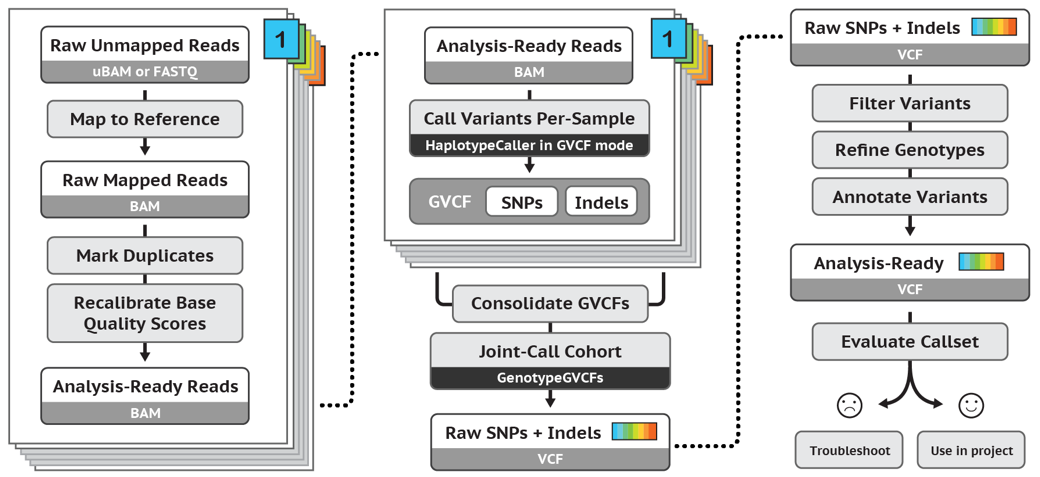
\includegraphics[width=0.8\textwidth]{gatk_varcall_workflow.png}
\caption{Variant calling best practices, from GATK.}
\label{fig:gatk-varcall-workflow}
\end{figure}

\subsection{Prerequisites}

I wish to give a general workflow first for when you, the audience, shall use this workflow in your own research project. The ``raw materials'' are short-read sequencing data and a reference genome. If you are doing this in a lab, the sequencing data is given from the experiment (well duh!). The reference genome, on the other hand, can be found in the \href{https://www.ncbi.nlm.nih.gov/datasets/}{NCBI Datasets}. Enter a species name, and scroll down to download its reference genome (try it!).


For example, the reference genome of a common strain of \textit{E. coli}, O157:H7, can be found through searching NCBI Datasets (\href{https://www.ncbi.nlm.nih.gov/datasets/taxonomy/83334/}{you should find this page}). You can download the genome and find a \texttt{.fna} file starting with this

\begin{minted}[breaklines]{text}
>NC_002695.2 Escherichia coli O157:H7 str. Sakai DNA, complete genome
AGCTTTTCATTCTGACTGCAACGGGCAATATGTCTCTGTGTGGATTAAAAAAAGAGTCTCTGACAGCAGCTTCTGAACTG
GTTACCTGCCGTGAGTAAATTAAAATTTTATTGACTTAGGTCACTAAATACTTTAACCAATATAGGCATAGCGCACAGAC
AGATAAAAATTACAGAGTACACAACATCCATGAAACGCATTAGCACCACCATTACCACCACCATCACCACCACCATCACC
ATTACCATTACCACAGGTAACGGTGCGGGCTGACGCGTACAGGAAACACAGAAAAAAGCCCGCACCTGACAGTGCGGGCT
...
\end{minted}

Here, the line starting with \texttt{>} is an information line about the sequence that follows and does not contain the genome (obviously). There, \texttt{NC\_002695.2} is a reference number that can can find this genome with on NCBI. Indeed, typing this number into a search box on the NCBI website, we can find \href{https://www.ncbi.nlm.nih.gov/nuccore/NC_002695.2/}{this page}, which shows us all the information about this reference genome. Take a moment to explore what information this page has.

\subsection{Data formats}

The above \textit{E. coli} reference genome is in the \textit{FASTA format}. There are only a couple of important formats for genome information (\href{https://www.animalgenome.org/bioinfo/resources/manuals/seqformats}{See this link}). Importantly, all these formats are in plain text, so you can open them up in a text editor and see. You should familiarize yourself with these formats, because each of these formats can manifest itself in different file suffixes. For example, the file containing the above \textit{E. coli} sequence ends in \texttt{.fna} to indicate that it is a reference genome, but the format of its content doesn't differ from an ordinary \textit{FASTA} file a bit and don't need to be handled differently in a software. Common filename extensions for the FASTA format are \texttt{.fasta}, \texttt{.fa}, and \texttt{.fna}.

An extension of the \textit{FASTA} format is the \textit{FASTQ} format, where the \textit{Q} stands for ``quality''. It is a format designed for raw results from genome sequencing, where in addition to the sequence of each read, there is also a confidence for the quality of each nucleotide in each read. You can find details on the FASTQ format \href{https://en.wikipedia.org/wiki/FASTQ_format}{on Wikipedia}. Different sequencing platforms could have different specialized formats, but FASTQ is a good starting point and the format used by the widely popular Illumina sequencers.

\section{Practice}

You should have the following softwares installed as assignment from the last workshop. Depending on how you formatted your \texttt{\$PATH} (see Workshop 1 if you are not familiar), the exact commands invoking these softwares might be different, so I will also note the format of invoking these softwares during this tutorial.

\begin{itemize}
   \item fastp. \texttt{fastp ...}
   \item BWA. \texttt{bwa ...}
   \item Samtools. \texttt{samtools ...}
   \item GATK. \texttt{gatk ...}
   \item Picard tools. It turns out that since the release of GATK4, Picard tools are included inside of gatk. So the commands to invoke the Picard tools is also \texttt{gatk ...}
   \item Tablet. This is a GUI-based software so as long as you can open it, we are good.
\end{itemize}

On a separate note, all the above tools but Picard happens to be on Bioconda, so they can be quite easily installed with Conda or its faster derivative Mamba after \href{https://bioconda.github.io/}{setting up the Bioconda channel}, using the command

\texttt{mamba create -n biobyte-workshop samtools fastp bwa gatk4}

I have held back from mentioning environment management until the Python workshop, but this is a nice peek ahead.


\subsection{Example data}

For this tutorial, we will use the \href{https://www.ncbi.nlm.nih.gov/sra}{NCBI Sequencing Read Archive (SRA)} to find example data. SRA is an open repository of genome sequence data from experiments. Arbitrarily, I have selected \href{https://www.ncbi.nlm.nih.gov/sra/SRR7262824}{the run with accession SRR7262824} as our data today. You can download the sequencing data directly from NCBI, and I have also \href{https://duke.box.com/s/jtu2wv1agbo2kp60z0k1mt9oos9b8v1k}{uploaded it on Box} for faster downloads. Either way, you should end up with a file \texttt{SRR7262824.fastq.gz}. For sake of clarity, rename this file to \texttt{reads.fastq.gz}.

This run is concerning \textit{E. coli O157:H7}, so we should also fetch its \href{https://www.ncbi.nlm.nih.gov/datasets/taxonomy/83334/}{reference genome}. Upon unzipping the file you downloaded from NCBI, you should eventually come upon two files, one starting with \texttt{GCF} and one starting with \texttt{GCA}. There are minor differences between the genomes in these two folders (detailed on \href{https://www.ncbi.nlm.nih.gov/assembly/model/}{this page}). We shall use the one starting with \texttt{GCF} (i.e. \texttt{GCF\_000008865.2\_ASM886v2\_genomic.fna}). Rename this reference file to \texttt{reference.fna}. Put \texttt{reads.fastq.gz} and \texttt{reference.fna} in the same folder. Start a terminal inside this folder, and we shall begin.

\subsection{Quality control}

\begin{enumerate}
   \item See \href{https://github.com/OpenGene/fastp}{the documentation for fastp} for all that it does. \begin{minted}[breaklines]{text}
   fastp -i reads.fastq.gz -o reads-processed.fastq.gz
   \end{minted}
\end{enumerate}

\subsection{Sequence alignment}

\subsubsection{Indexing the reference genome}

\begin{enumerate}
   \item \begin{minted}[breaklines]{text}
   bwa index reference.fna
   \end{minted}
   \item \begin{minted}[breaklines]{text}
   samtools faidx reference.fna
   \end{minted}
   \item \begin{minted}[breaklines]{text}
   gatk CreateSequenceDictionary REFERENCE=reference.fna OUTPUT=reference.dict
   \end{minted}
\end{enumerate}

\subsubsection{Alignment}

\begin{enumerate}
   \item Run BWA either single-threaded or multi-threaded. Multi-threaded is significantly faster, but single-threaded execution still completes within a reasonable amount of time due to the small size of the data we are dealing with.
   \begin{itemize}
      \item Single-threaded:
      \begin{minted}[breaklines]{text}
      bwa mem reference.fna reads-processed.fastq.gz > aligned.sam
      \end{minted}
      \item Multi-threaded (look up ``command substitution '' for what \texttt{\$(nproc)} means):
      \begin{minted}[breaklines]{text}
      bwa mem -t $(nproc) reference.fna reads-processed.fastq.gz > aligned.sam
      \end{minted}
   \end{itemize}
\end{enumerate}

\subsubsection{Post alignment}

\begin{enumerate}
   \item Convert SAM file to a more efficient BAM file (B stands for binary). \begin{minted}[breaklines]{text}
   samtools view  -S -b aligned.sam > aligned.bam
   \end{minted}
   \item Sort BAM file. \begin{minted}[breaklines]{text}
   samtools sort aligned.bam -o aligned-sorted.bam
   \end{minted}
   \item Index BAM file. \begin{minted}[breaklines]{text}
   samtools index aligned-sorted.bam
   \end{minted}
   \item View the resulting alignment (\texttt{aligned-sorted.bam}) with Tablet or some other alignment viewer.
\end{enumerate}

\subsection{Variant calling}

\begin{enumerate}
   \item Re-labeling the read groups. Not essential to the variant calling process but good practice.  \begin{minted}[breaklines]{text}
   gatk AddOrReplaceReadGroups I=aligned-sorted.bam O=aligned-rg.bam RGID=1 RGLB=A RGPL=Illumina RGPU=MiSeq RGSM=1
   \end{minted}
   \item Mark duplicates. \begin{minted}[breaklines]{text}
   gatk MarkDuplicates I=aligned-rg.bam O=aligned-md.bam M=aligned-metrics.txt
   \end{minted}
   \item Index the resulting file. \begin{minted}[breaklines]{text}
   samtools index aligned-md.bam
   \end{minted}
   \item Run HaplotypeCaller to identify the variants in our sequencing data. \begin{minted}[breaklines]{text}
   gatk HaplotypeCaller --native-pair-hmm-threads $(nproc) -R reference.fna -I aligned-md.bam -O aligned.g.vcf
   \end{minted}
   (took 3.4 minutes on my computer)
   \item Open the resulting \texttt{aligned.g.vcf} with a spreadsheet viewer such as Microsoft Excel. This is a tab-separated file.
\end{enumerate}

\section{Additional thoughts}

\subsection{}

If you have multiple sequencing runs that you want to compare against each other, the following commands will let you create multiple variant calls and merge them together:

\begin{enumerate}
   \item Run the HaplotypeCaller for each sequencing run that you will to include in the comparison, producing files like \texttt{aligned1-md.bam}, \texttt{aligned2-md.bam}, ...
   \item Combine the alignments into a genomics database (GenomicsDB). \begin{minted}[breaklines]{text}
   gatk GenomicsDBImport -V aligned1-md.bam -V aligned2-md.bam ... --genomics-workspace-path combined -L “reference-interval”
   \end{minted}
   \item Export the GenomicsDB into a VCF file. \begin{minted}[breaklines]{text}
   gatk GenotypeGVCFs -R reference.txt -V -gendb://combined -O combined.vcf
   \end{minted}
   \item View the resulting VCF file with a spreadsheet viewer.
\end{enumerate}

\subsection{}

If the sequence data that you have is very large, you may consider running the commands on a remote server such that you can leave the execution running and come back later. In this case, the tool \href{https://www.gnu.org/software/screen/}{GNU screen} can be very helpful. GNU screen allows you do exit out of a SSH terminal session while still keeping the terminal running.

\subsection{}

If you have a lot of sequencing data that want to process in batch (e.g. when variant calling for multiple sequence runs), you may consider using a bash script to automate the whole process. A good starting point can be this script in my GitHub: \href{https://github.com/longyuxi/dew-lover/blob/master/align.sh}{longyuxi/dew-lover/align.sh}.



\end{document}
